\chapter{Fundamentação Teórica}\label{cap:fundamentacao}

Este capítulo apresenta os fundamentos teóricos para compreender o problema de planejamento de caminhos em robótica, com ênfase em métodos baseados em amostragem. São introduzidos os conceitos de espaço de configuração e espaço livre, que modelam o problema como uma busca por conectividade em um espaço contínuo.

O problema é então formulado matematicamente, distinguindo planejamento geométrico de caminhos, planejamento de trajetórias e planejamento cinodinâmico. A partir dessa formulação, são apresentadas diferentes classes de algoritmos, com destaque para métodos probabilísticos baseados em árvores: RRT, RRT-Connect, RRT* e EST.

Por fim, são discutidas propriedades formais desses planejadores, como completude probabilística e otimalidade assintótica, e suas diferenças em relação à variante híbrida proposta neste trabalho.

\section{Planejamento de caminho em robótica}\label{sec:planejamento_caminho}

O planejamento de caminho é um dos problemas centrais da robótica móvel e da manipulação robótica que consiste em determinar uma sequência contínua de configurações que leve o robô de um estado inicial a um objetivo sem violar restrições do ambiente. Conforme discutido por \citet{choset2005principles}, o problema pode ser interpretado como uma busca geométrica em um espaço de estados contínuo, no qual obstáculos induzem regiões proibidas e o movimento deve respeitar restrições cinemáticas e, eventualmente, dinâmicas.

Diferente do controle de movimento, que trata da execução física das ações, o planejamento opera em nível deliberativo: abstrai a dinâmica e foca na viabilidade geométrica do trajeto. Isso permite modelar o problema matematicamente, transformando a navegação em uma questão de conectividade topológica.

A formulação clássica assume conhecimento prévio do ambiente e abordagem determinística, onde o objetivo é encontrar um caminho contínuo no espaço livre que conecte duas configurações válidas.

\section{Espaço de configuração e espaço livre}
\label{sec:espaco_configuracao}

Para formalizar o planejamento de caminho, introduz-se o conceito de \textbf{espaço de configuração}, denotado por $Q$. Conforme \citet{choset2005principles}, $Q$ representa o conjunto de todas as configurações possíveis do robô, onde cada ponto descreve completamente o estado geométrico do sistema. Com isso, um robô de geometria arbitrária é reduzido a um ponto em $Q$, simplificando a representação do problema.

Uma \textbf{configuração} $q$ é um vetor de parâmetros que especifica univocamente a posição e orientação de cada ponto do robô no espaço de trabalho. A dimensão de $Q$ corresponde ao número de graus de liberdade do sistema.

Para um robô rígido planar, o espaço de configuração é:

\begin{equation}
    Q = \mathbb{R}^2 \times S^1,
    \label{eq:cspace_planar}
\end{equation}

onde $\mathbb{R}^2$ representa a posição no plano e $S^1$ a orientação angular. Para um manipulador com $n$ juntas de revolução, tem-se $Q = (S^1)^n$~\cite{choset2005principles}.

Considere um \textbf{espaço de trabalho} $W \subset \mathbb{R}^d$, com $d \in \{2, 3\}$, contendo obstáculos $W_{O_i}$. O conjunto livre no espaço de trabalho é

\begin{equation}
    W_{\mathrm{free}} = W \setminus \bigcup_i W_{O_i}.
    \label{eq:wfree}
\end{equation}

O planejamento não ocorre diretamente no espaço de trabalho, mas no espaço de configuração. Seja $R(q) \subset W$ o conjunto de pontos ocupados pelo robô na configuração $q \in Q$. O conjunto de configurações em colisão com o obstáculo $W_{O_i}$ é

\begin{equation}
    Q_{O_i} = \bigl\{ q \in Q \mid R(q) \cap W_{O_i} \neq \emptyset \bigr\},
    \label{eq:qobs}
\end{equation}

e o \textbf{espaço livre de configurações} é

\begin{equation}
    Q_{\mathrm{free}} = Q \setminus \bigcup_i Q_{O_i}.
    \label{eq:qfree}
\end{equation}

Obstáculos simples no espaço de trabalho podem induzir regiões proibidas de geometria complexa em $Q$, tornando inviável construí-las explicitamente para robôs com muitos graus de liberdade~\cite{choset2005principles}. Os algoritmos baseados em amostragem contornam isso consultando $Q_{O_i}$ apenas pontualmente, via verificadores de colisão, sem construir $Q_{\mathrm{free}}$ por completo~\cite{choset2005principles, lavalle2006planning}.

Assim, o planejamento de caminho passa a ser uma busca no espaço de configuração livre: encontrar uma sequência contínua de configurações válidas em $Q_{\mathrm{free}}$ que conecte configuração inicial e objetivo.

\section{Formulação matemática do planejamento de caminhos}
\label{sec:formulacao}

A partir de $Q$ e $Q_{\mathrm{free}} \subset Q$, o problema de planejamento pode ser formulado como um problema de conectividade em um espaço topológico contínuo~\cite{choset2005principles}: determinar um caminho contínuo que conecte duas configurações válidas sem interceptar regiões proibidas.

Sejam $q_{\mathrm{start}}, q_{\mathrm{goal}} \in Q_{\mathrm{free}}$ duas configurações admissíveis. Um \textbf{caminho} é uma função contínua

\begin{equation}
    c : [0,1] \rightarrow Q,
    \label{eq:path_mapping}
\end{equation}

tal que

\begin{equation}
    c(0) = q_{\mathrm{start}}, \qquad
    c(1) = q_{\mathrm{goal}}, \qquad
    c(s) \in Q_{\mathrm{free}}, \;\forall s \in [0,1].
    \label{eq:path_conditions}
\end{equation}

A solução consiste em encontrar $c \in C^0$ satisfazendo a \autoref{eq:path_conditions}, ou concluir que não existe.

\subsection*{Problema de viabilidade}

A formulação mais básica, o \textbf{problema de viabilidade}, busca apenas a existência de um caminho livre de colisão: dados $q_{\mathrm{start}}, q_{\mathrm{goal}} \in Q_{\mathrm{free}}$, determinar $c : [0,1] \rightarrow Q$ satisfazendo \autoref{eq:path_conditions}, ou concluir que nenhuma solução existe~\citep{choset2005principles}.

\subsection*{Problema de planejamento ótimo}

Quando não basta encontrar qualquer caminho viável, é necessário otimizar algum critério. Seja

\begin{equation}
    \Sigma_{\mathrm{free}} =
    \left\{
        c : [0,1] \rightarrow Q \;\middle|\;
        c \in C^0,\;
        c(0) = q_{\mathrm{start}},\;
        c(1) = q_{\mathrm{goal}},\;
        c(s) \in Q_{\mathrm{free}},\; \forall s \in [0,1]
    \right\}
    \label{eq:admissible_paths}
\end{equation}

o conjunto de caminhos admissíveis, e

\begin{equation}
    J : \Sigma_{\mathrm{free}} \rightarrow \mathbb{R}_{\geq 0}
    \label{eq:functional_cost}
\end{equation}

uma função de custo. O problema ótimo consiste em determinar

\begin{equation}
    c^* = \arg\min_{c \in \Sigma_{\mathrm{free}}} J(c),
    \label{eq:optimal_planning_problem}
\end{equation}

conforme formalizado em \cite{Karaman2011SamplingbasedAF}.

Como os planejadores baseados em amostragem produzem sequências finitas de configurações, o custo é tratado em forma discreta. Dado o caminho $q_0, q_1, \ldots, q_m$, com $q_0 = q_{\mathrm{start}}$ e $q_m = q_{\mathrm{goal}}$:

\begin{equation}
    J(c) =
    \sum_{i=0}^{m-1}
    d(q_i, q_{i+1}),
    \label{eq:discrete_path_cost}
\end{equation}

onde $d(q_i, q_{i+1})$ é a distância entre configurações consecutivas. Em espaços euclidianos:

\begin{equation}
    d(q_i, q_{i+1}) =
    \| q_{i+1} - q_i \|.
    \label{eq:euclidean_distance}
\end{equation}

Outros critérios possíveis incluem tempo, consumo de energia, suavidade da trajetória ou distância a obstáculos~\cite{choset2005principles}.

\subsection*{Planejamento de trajetória e planejamento cinodinâmico}

Quando a solução é parametrizada no tempo, passa-se a tratar de uma trajetória. A configuração torna-se uma função temporal:

\begin{equation}
    q : [0,T] \rightarrow Q,
\end{equation}

descrevendo não apenas a sequência de configurações, mas como elas são percorridas ao longo do tempo. Em formulações mais gerais, o estado do sistema inclui velocidades:

\begin{equation}
    x(t) = (q(t), \dot{q}(t)),
\end{equation}

com evolução descrita por

\begin{equation}
    \dot{x}(t) = f(x(t), u(t)), \qquad u(t) \in \mathcal{U},
    \label{eq:system_dynamics}
\end{equation}

onde $u(t)$ é a entrada de controle e $\mathcal{U}$ o conjunto de controles admissíveis. Quando o planejamento deve satisfazer esse modelo, respeitando restrições de velocidade, aceleração e atuação, o problema é denominado planejamento cinodinâmico~\cite{LaValle1999RandomizedKP}.

Neste trabalho, considera-se apenas o planejamento geométrico de caminhos. A evolução temporal e as restrições dinâmicas são abstraídas, reduzindo o problema à busca por conectividade em $Q_{\mathrm{free}}$.

\section{Algoritmos de planejamento de caminhos}
\label{sec:algoritmos}

Uma vez formulado o problema como busca por curva contínua em $Q_{\mathrm{free}}$, diferentes estratégias podem ser empregadas para resolvê-lo. Conforme \citet{choset2005principles}, os métodos se dividem em: (i) busca em grafos discretizados, (ii) decomposição do espaço livre e (iii) métodos probabilísticos baseados em amostragem.

Em espaços de baixa dimensão, é viável construir grafos ou estruturas geométricas explícitas. À medida que a dimensão cresce, representar $Q_{\mathrm{free}}$ explicitamente torna-se proibitivo, motivando o uso de métodos baseados em amostragem.

\subsection{Métodos clássicos}

\paragraph{Busca em grafos discretizados:}
Com o espaço discretizado, o problema vira uma busca em grafos. Algoritmos como Dijkstra e A* garantem completude, mas o número de estados cresce exponencialmente com a dimensão.

\paragraph{Decomposição celular:}
$Q_{\mathrm{free}}$ é particionado em células disjuntas e um grafo de adjacência é construído entre elas. Se existir uma sequência de células conectando $q_{\mathrm{start}}$ a $q_{\mathrm{goal}}$, um caminho pode ser obtido~\cite{choset2005principles}.

\paragraph{Roadmaps determinísticos:}
O grafo de visibilidade e o diagrama de Voronoi generalizado são exemplos clássicos. O diagrama de Voronoi maximiza o afastamento em relação a obstáculos, mas sua construção exata é custosa com muitos graus de liberdade, o que impulsionou o desenvolvimento dos métodos probabilísticos.

\subsection{Métodos probabilísticos baseados em amostragem}

Esses métodos não constroem $Q_{\mathrm{free}}$ explicitamente. Em vez disso, geram amostras aleatórias em $Q$ e usam verificações locais de colisão para construir incrementalmente uma estrutura de conectividade.

Conforme \citet{choset2005principles}, são tipicamente \textit{probabilisticamente completos}: se existe um caminho com folga positiva em relação aos obstáculos, a probabilidade de encontrá-lo converge para 1 com o aumento do número de amostras.

Dois paradigmas principais são identificados:

\begin{itemize}
    \item \textbf{Roadmaps probabilísticos (PRM)};
    \item \textbf{Planejadores baseados em árvores} (RRT, EST).
\end{itemize}

Neste trabalho, o foco recai sobre os planejadores baseados em árvores.

\subsection{Amostragem e viés de exploração}
\label{subsec:amostragem_vies}

Nos planejadores baseados em amostragem, como novas configurações são geradas influencia diretamente a busca. Em geral, uma amostra $q_{\mathrm{rand}}$ é gerada no espaço de configuração e o algoritmo decide onde expandir sua estrutura a partir dela. A distribuição das amostras afeta tanto a exploração global quanto a eficiência em regiões de difícil acesso.

A estratégia mais direta é a amostragem uniforme, na qual todos os pontos têm igual probabilidade de seleção. Favorece a exploração global, mas em ambientes com passagens estreitas, a chance de amostrar exatamente nessas regiões pode ser baixa.

Uma alternativa comum é o viés em direção ao objetivo, onde $q_{\mathrm{goal}}$ é escolhido com probabilidade $p_{\mathrm{goal}}$:

\begin{equation}
q_{\mathrm{rand}} =
\begin{cases}
q_{\mathrm{goal}}, & \text{com probabilidade } p_{\mathrm{goal}}, \\
\textsc{Sample}(Q), & \text{com probabilidade } 1 - p_{\mathrm{goal}}.
\end{cases}
\label{eq:goal_bias}
\end{equation}

Em ambientes simples, isso acelera a convergência. Porém, com obstáculos entre a árvore e o objetivo, um $p_{\mathrm{goal}}$ elevado tende a gerar mais tentativas inválidas, já que o planejador insiste em direções bloqueadas.

Além do viés em direção ao objetivo, a forma de selecionar amostras e expandir novos vértices altera significativamente a distribuição dos nós, como ilustrado na Figura~\ref{fig:comparacao_rrt_amostragem}.

\begin{figure}[H]
    \centering
    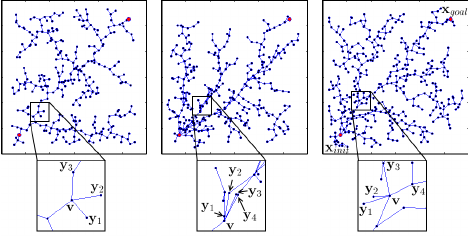
\includegraphics[width=0.75\textwidth]{tcc/Cap02/img/image1.png}
    \caption{Comparação entre árvores RRT geradas a partir de diferentes estratégias de planejamento e amostragem. Diferentes formas de expansão influenciam a distribuição dos nós e a cobertura do espaço de configuração. Fonte: \citep{park2014poissonrrt}.}
    \label{fig:comparacao_rrt_amostragem}
\end{figure}

No RRT, um mecanismo importante é o \textbf{viés de Voronoi}. Dada uma árvore $T$ com vértices $q_1, \ldots, q_n$, a região de Voronoi de $q_i$ é o conjunto de pontos mais próximos dele do que de qualquer outro vértice:

\begin{equation}
V(q_i) =
\left\{
q \in Q_{\mathrm{free}} \mid
d(q,q_i) \leq d(q,q_j), \; \forall j \neq i
\right\}.
\label{eq:voronoi_region}
\end{equation}

A Figura~\ref{fig:voronoi_rrt} ilustra essas regiões em uma árvore RRT. Regiões maiores, geralmente nas extremidades da árvore, indicam vértices com maior probabilidade de serem selecionados.

\begin{figure}[H]
    \centering
    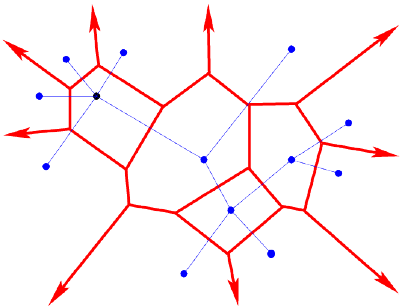
\includegraphics[width=0.65\textwidth]{tcc/Cap02/img/image2.png}
    \caption{Representação conceitual das regiões de Voronoi associadas aos vértices de uma árvore RRT. Regiões maiores possuem maior probabilidade de seleção durante a expansão. Fonte: \citep{arnold2013convexhull}.}
    \label{fig:voronoi_rrt}
\end{figure}

Quando $q_{\mathrm{rand}}$ é gerada uniformemente, o vértice mais próximo é selecionado para expansão. Vértices com regiões de Voronoi maiores têm maior chance de seleção, proporcional à medida de sua região:

\begin{equation}
P(q_i \text{ ser selecionado}) =
\frac{\mu(V(q_i))}{\mu(Q_{\mathrm{free}})},
\label{eq:voronoi_bias}
\end{equation}

onde $\mu(V(q_i))$ é a medida da região de $q_i$ e $\mu(Q_{\mathrm{free}})$ a medida total do espaço livre. O RRT tende, assim, a expandir naturalmente em direção a regiões ainda pouco exploradas.

O EST funciona de forma diferente. Em vez de selecionar o vértice mais próximo de uma amostra global, escolhe um nó com base em estimativa de densidade local. Nós em regiões menos densas recebem maior probabilidade de expansão, com peso

\begin{equation}
w(q_i) = \frac{1}{\rho(q_i) + \varepsilon},
\label{eq:est_weight}
\end{equation}

onde $\rho(q_i)$ estima a densidade ao redor de $q_i$ e $\varepsilon > 0$ evita divisão por zero. A probabilidade de seleção é

\begin{equation}
P(q_i) =
\frac{w(q_i)}
{\sum_{q_j \in T} w(q_j)}.
\label{eq:est_probability}
\end{equation}

O RRT tem viés implícito pelo diagrama de Voronoi; o EST controla explicitamente a densidade para favorecer regiões menos cobertas. Essa distinção é importante para a variante híbrida proposta, que combina esses dois mecanismos.

\subsection{Rapidly-exploring Random Trees (RRT)}
\label{subsec:rrt}

O RRT, introduzido por \citet{lavalle1998rapidly} e descrito em \citet{choset2005principles}, constrói incrementalmente uma árvore enraizada em $q_{\mathrm{start}}$, expandindo em direção a amostras aleatórias do espaço de configuração.

Como discutido na Seção~\ref{subsec:amostragem_vies}, vértices com maiores regiões de Voronoi associadas têm maior probabilidade de seleção, o que leva o RRT a explorar regiões ainda pouco cobertas sem nenhuma lógica explícita de densidade.

\begin{algorithm}[H]
\caption{RRT}
\begin{algorithmic}[1]
\State $T \gets \{q_{\mathrm{start}}\}$
\While{não atingir critério de parada}
    \State $q_{\mathrm{rand}} \gets \textsc{Sample}(Q)$
    \State $q_{\mathrm{near}} \gets \textsc{Nearest}(T, q_{\mathrm{rand}})$
    \State $q_{\mathrm{new}} \gets \textsc{Steer}(q_{\mathrm{near}}, q_{\mathrm{rand}})$
    \If{$\textsc{CollisionFree}(q_{\mathrm{near}}, q_{\mathrm{new}})$}
        \State adicionar $q_{\mathrm{new}}$ e aresta correspondente a $T$
    \EndIf
\EndWhile
\end{algorithmic}
\end{algorithm}

O RRT é probabilisticamente completo sob hipóteses de existência de caminho com folga positiva, mas não é assintoticamente ótimo.

\subsection{RRT-Connect}

Proposto por \citet{kuffner2000rrtconnect}, o RRT-Connect mantém duas árvores: uma enraizada em $q_{\mathrm{start}}$ e outra em $q_{\mathrm{goal}}$. A cada iteração, uma árvore é expandida em direção a uma amostra aleatória, enquanto a outra tenta se conectar ao novo vértice gerado, de forma mais agressiva do que no RRT tradicional, com expansões repetidas enquanto a conexão for válida. Na prática, isso reduz o número de iterações necessárias em cenários onde as duas regiões podem ser ligadas por expansões locais viáveis.

\subsection{RRT*}

O RRT* foi introduzido por \citet{Karaman2011SamplingbasedAF} como uma modificação do RRT com garantia de \textbf{otimalidade assintótica}. Além da expansão incremental, inclui uma etapa de reconexão local (\textit{rewiring}): vértices vizinhos são reconectados caso isso reduza o custo total do caminho desde a raiz.

\begin{algorithm}[H]
\caption{RRT*}
\begin{algorithmic}[1]
\State $T \gets \{q_{\mathrm{start}}\}$
\While{não atingir critério de parada}
    \State $q_{\mathrm{rand}} \gets \textsc{Sample}(Q)$
    \State $q_{\mathrm{near}} \gets \textsc{Nearest}(T, q_{\mathrm{rand}})$
    \State $q_{\mathrm{new}} \gets \textsc{Steer}(q_{\mathrm{near}}, q_{\mathrm{rand}})$
    \If{$\textsc{CollisionFree}(q_{\mathrm{near}}, q_{\mathrm{new}})$}
        \State determinar conjunto de vizinhos $\mathcal{Q}_{\mathrm{near}}$
        \State escolher pai de menor custo para $q_{\mathrm{new}}$
        \State reconectar vizinhos se houver redução de custo
    \EndIf
\EndWhile
\end{algorithmic}
\end{algorithm}

O RRT* é simultaneamente probabilisticamente completo e assintoticamente ótimo.

\subsection{Expansive Space Trees (EST)}
\label{subsec:est}

O EST é um planejador baseado em árvores que expande preferencialmente regiões pouco densamente amostradas~\cite{choset2005principles}. Não usa amostras aleatórias globais nem o critério do vértice mais próximo: a seleção é guiada por uma estimativa de densidade local, e a nova configuração é gerada por perturbação aleatória a partir do nó escolhido.

O objetivo é evitar que a árvore cresça repetidamente em regiões já exploradas. Nós em regiões menos densas recebem maior probabilidade de seleção. Se a conexão for livre de colisão, o vértice é adicionado à árvore.

\begin{algorithm}[H]
\caption{EST}
\begin{algorithmic}[1]
\State $T \gets \{q_{\mathrm{start}}\}$
\While{não atingir critério de parada}
    \State selecionar $q \in T$ com probabilidade inversamente proporcional à densidade local
    \State gerar $q_{\mathrm{new}}$ por perturbação aleatória
    \If{$\textsc{CollisionFree}(q, q_{\mathrm{new}})$}
        \State adicionar $q_{\mathrm{new}}$ a $T$
    \EndIf
\EndWhile
\end{algorithmic}
\end{algorithm}

Sob hipóteses de expansividade do espaço livre, o EST é probabilisticamente completo.

\subsection{Síntese dos algoritmos apresentados}
\label{subsec:sintese_algoritmos}

Os três algoritmos diferem principalmente no critério de expansão e nas garantias teóricas. O RRT explora rapidamente pelo viés de Voronoi. O RRT* acrescenta reconexão orientada por custo. O EST distribui a exploração com base em densidade local, sem atração global explícita.

\begin{table}[H]
\centering
\caption{Comparação conceitual entre RRT e EST}
\label{tab:comparacao_rrt_est}
\begin{tabular}{@{}p{4cm}p{5cm}p{5cm}@{}}
\toprule
\textbf{Aspecto} & \textbf{RRT} & \textbf{EST} \\ \midrule
Estrutura de busca & Árvore incremental & Árvore incremental \\
Critério de expansão & Expansão em direção a amostra aleatória & Seleção de nós por densidade local \\
Mecanismo de exploração & Viés de Voronoi implícito & Priorização de regiões pouco densas \\
Probabilidade de seleção & Proporcional ao tamanho da região de Voronoi & Inversamente proporcional à densidade local \\
Geração de novos nós & Direcionada por $q_{\mathrm{rand}}$ & Perturbação aleatória local \\
Vantagem principal & Exploração rápida do espaço & Cobertura equilibrada do espaço livre \\
Limitação & Muitas colisões em regiões obstruídas & Lento em grandes espaços abertos \\ \bottomrule
\end{tabular}
\end{table}

A variante híbrida proposta neste trabalho busca combinar a força de exploração global do RRT com o controle de densidade do EST, aproveitando o que cada um tem de melhor.

\section{Propriedades formais dos planejadores}
\label{sec:propriedades_formais}

Os algoritmos de planejamento podem ser comparados por propriedades formais relacionadas à existência de solução, à capacidade de encontrá-la e à qualidade do caminho obtido. Essas propriedades complementam a avaliação experimental, pois descrevem o comportamento do algoritmo no limite.

Esta seção não reproduz as provas formais da literatura. O foco é apresentar os principais argumentos por trás da completude probabilística e da otimalidade assintótica, no contexto dos algoritmos discutidos.

\subsection{Completude probabilística no RRT e no EST}
\label{subsec:completude_rrt_est}

Embora ambos sejam probabilisticamente completos, RRT e EST chegam a essa garantia por caminhos distintos. No RRT, o argumento parte da existência de um caminho com folga positiva em relação aos obstáculos. No EST, é necessário assumir que o espaço livre possui propriedades de expansividade.

Seja $A_k$ o evento de que o planejador encontrou solução após $k$ iterações. A completude probabilística exige que

\begin{equation}
    \lim_{k \rightarrow \infty} \mathbb{P}(A_k) = 1,
    \label{eq:def_completude_probabilistica}
\end{equation}

ou, equivalentemente, que a probabilidade de falha vá a zero:

\begin{equation}
    \lim_{k \rightarrow \infty} \mathbb{P}(A_k^c) = 0.
    \label{eq:def_falha_probabilistica}
\end{equation}

\paragraph{Ideia da prova para o RRT:}

Kleinbort et al.~\cite{kleinbort2022probabilisticcompletenessrrtgeometric} demonstram a completude sob a hipótese de existência de solução com folga positiva $\delta > 0$, que garante uma vizinhança ao redor do caminho inteiramente em $Q_{\mathrm{free}}$.

Dado um caminho válido $\pi$, essa folga permite cobri-lo por uma sequência finita de bolas abertas:

\begin{equation}
    B_0, B_1, \ldots, B_m,
    \label{eq:rrt_cobertura_bolas}
\end{equation}

com $B_0$ contendo $q_{\mathrm{start}}$, $B_m$ intersectando a região objetivo e todas as bolas em $Q_{\mathrm{free}}$. Em vez de analisar o caminho contínuo, a prova considera essa sequência finita de regiões que a árvore precisa alcançar.

Assumindo $Q$ mensurável com $0 < \mu(Q) < \infty$, a probabilidade de uma amostra uniforme cair em $B_{i+1}$ é

\begin{equation}
    p_i = \frac{\mu(B_{i+1})}{\mu(Q)} > 0.
    \label{eq:probabilidade_avanco_rrt}
\end{equation}

Como cada bola tem medida positiva, $p_i > 0$. Se a amostra cair em $B_{i+1}$ e o operador de expansão produzir uma conexão compatível com a folga, o segmento permanece em $Q_{\mathrm{free}}$.

O Algoritmo~\ref{alg:prova_completude_rrt} resume esse argumento.

\begin{algorithm}[H]
\caption{Esquema de prova da completude probabilística do RRT}
\label{alg:prova_completude_rrt}
\begin{algorithmic}[1]
\State \textbf{Entrada:} caminho viável $\pi$ com folga $\delta > 0$
\State \textbf{Saída:} conclusão de que $\mathbb{P}(A_k) \rightarrow 1$
\State Cobrir $\pi$ por bolas $B_0, B_1, \ldots, B_m \subset Q_{\mathrm{free}}$
\For{$i \gets 0$ até $m-1$}
    \State Assumir que $T$ já alcançou $B_i$
    \State $p_i \gets \dfrac{\mu(B_{i+1})}{\mu(Q)}$; como $\mu(B_{i+1}) > 0$, então $p_i > 0$
\EndFor
\State Alcançar o objetivo requer uma sequência finita de avanços com probabilidade positiva
\State Logo, a probabilidade de falhar indefinidamente tende a zero
\State Concluir: $\lim_{k \to \infty}\mathbb{P}(A_k)=1$
\end{algorithmic}
\end{algorithm}

Kleinbort et al.~\cite{kleinbort2022probabilisticcompletenessrrtgeometric} mostram ainda que a probabilidade de falha decai exponencialmente:

\begin{equation}
    \mathbb{P}(A_k^c) \leq a e^{-bk},
    \label{eq:falha_exponencial_rrt}
\end{equation}

com $a, b > 0$. Como $e^{-bk} \rightarrow 0$, a completude probabilística está estabelecida.

\paragraph{Ideia da prova para o EST:}

O argumento do EST segue linha diferente. O algoritmo não expande a partir do vértice mais próximo de uma amostra global, então a prova não pode se apoiar diretamente na medida das bolas ao longo de um caminho. Em vez disso, depende da hipótese de que o espaço livre é expansivo: regiões já alcançadas têm visibilidade suficiente para permitir expansão em novas áreas, evitando que a árvore fique confinada em uma sub-região indefinidamente~\cite{hsu1997path,hsu1999path}.

O EST atribui a cada nó $q_i$ um peso inversamente proporcional à densidade local:

\begin{equation}
    w(q_i) = \frac{1}{\rho(q_i) + \varepsilon},
    \label{eq:peso_est_completude}
\end{equation}

com probabilidade de seleção

\begin{equation}
    P(q_i) = \frac{w(q_i)}{\sum_{q_j \in T} w(q_j)}.
    \label{eq:probabilidade_est_completude}
\end{equation}

Essa distribuição evita concentração excessiva em regiões já densas e mantém probabilidade positiva de expandir em áreas ainda pouco cobertas. Sob as hipóteses de Hsu et al.~\cite{hsu1997path,hsu1999path}, isso é suficiente para garantir que a árvore avance progressivamente pelo espaço livre.

O Algoritmo~\ref{alg:prova_completude_est} organiza esse argumento.

\begin{algorithm}[H]
\caption{Esquema de prova da completude probabilística do EST}
\label{alg:prova_completude_est}
\begin{algorithmic}[1]
\State \textbf{Entrada:} espaço livre expansivo e caminho viável
\State \textbf{Saída:} conclusão de que $\mathbb{P}(A_k) \rightarrow 1$
\State Pela hipótese de expansividade, identificar região livre visível a partir da parte já alcançada de $T$
\State Identificar nó útil $q_i \in T$ com densidade local baixa
\State Atribuir a $q_i$ probabilidade positiva pela distribuição da Equação~\ref{eq:probabilidade_est_completude}
\State Gerar perturbação local; se livre de colisão, a árvore avança para nova região
\State Repetir para uma sequência finita de regiões até o objetivo
\State Concluir: $\lim_{k \to \infty}\mathbb{P}(A_k)=1$
\end{algorithmic}
\end{algorithm}

O RRT se apoia na medida positiva das bolas ao longo de um caminho com folga. O EST depende de uma propriedade estrutural do espaço livre. A Tabela~\ref{tab:comparacao_completude_rrt_est} resume a comparação.

\begin{table}[H]
\centering
\caption{Comparação entre os argumentos de completude probabilística do RRT e do EST}
\label{tab:comparacao_completude_rrt_est}
\begin{tabular}{@{}p{3.5cm}p{5.5cm}p{5.5cm}@{}}
\toprule
\textbf{Aspecto} & \textbf{RRT} & \textbf{EST} \\ \midrule
Mecanismo de expansão & Vértice mais próximo de amostra aleatória & Nós selecionados por densidade local \\
Hipótese principal & Caminho com folga positiva e medida de Lebesgue $> 0$ & Condições de expansividade no espaço livre \\
Evento de sucesso & Amostra cair em região de medida positiva & Selecionar nó útil e gerar perturbação válida \\
Estrutura da prova & Cobertura por bolas e avanço sequencial & Expansão progressiva via controle de densidade \\
Garantia obtida & Completude probabilística & Completude probabilística sob expansividade \\ \bottomrule
\end{tabular}
\end{table}

Essa comparação é retomada no Capítulo~\ref{cap:metodologia}, onde a variante híbrida proposta é analisada sob as mesmas hipóteses.

\subsection{Otimalidade assintótica no RRT e no EST}
\label{subsec:otimalidade_rrt_est}

Completude probabilística não diz nada sobre a qualidade da solução encontrada. Um planejador pode ser completo e retornar caminhos longos ou irregulares sem nenhuma garantia de melhora. Para isso existe a propriedade de \textbf{otimalidade assintótica}.

Seja $c^*$ o custo ótimo e $c_k$ o custo da melhor solução após $k$ amostras. O planejador é assintoticamente ótimo quando, para qualquer $\varepsilon > 0$:

\begin{equation}
    \lim_{k \rightarrow \infty}
    \mathbb{P}\left(c_k - c^* < \varepsilon\right) = 1.
    \label{eq:otimalidade_assintotica_rrt_est}
\end{equation}

O RRT padrão não satisfaz essa propriedade. Cada vértice é conectado ao nó mais próximo sem considerar custo acumulado, e as conexões não são revisadas depois da inserção. Não há mecanismo que force a melhora progressiva dos caminhos encontrados.

O EST padrão tem a mesma limitação. Sua seleção por densidade favorece a cobertura do espaço, mas não é orientada por custo. Sem reconexão ou escolha de melhor pai, o algoritmo não converge para o ótimo.

Karaman e Frazzoli~\cite{Karaman2011SamplingbasedAF} mostram formalmente que RRT e EST não são assintoticamente ótimos em suas formulações originais, e propõem o RRT* como alternativa. A modificação central está em dois pontos: ao inserir um vértice, escolhe-se o vizinho que oferece menor custo acumulado desde a raiz, não o mais próximo; depois, os vértices vizinhos são verificados e reconectados se isso reduzir seus custos. A árvore não apenas cresce, mas continuamente melhora sua estrutura de custos.

A Tabela~\ref{tab:comparacao_otimalidade_rrt_est} resume a situação dos três algoritmos.

\begin{table}[H]
\centering
\caption{Comparação entre RRT, EST e RRT* quanto à otimalidade assintótica}
\label{tab:comparacao_otimalidade_rrt_est}
\begin{tabular}{@{}p{4cm}p{3.5cm}p{3.5cm}p{3.5cm}@{}}
\toprule
\textbf{Aspecto} & \textbf{RRT} & \textbf{EST} & \textbf{RRT*} \\ \midrule
Objetivo principal & Exploração rápida & Cobertura por densidade & Melhoria progressiva do custo \\
Critério de conexão & Vizinho mais próximo & Nó por densidade & Melhor pai entre vizinhos \\
Considera custo acumulado? & Não & Não & Sim \\
Possui \textit{rewiring}? & Não & Não & Sim \\
Melhora caminhos encontrados? & Não & Não & Sim \\
Completude probabilística & Sim & Sim, sob expansividade & Sim \\
Otimalidade assintótica & Não & Não & Sim \\ \bottomrule
\end{tabular}
\end{table}

Para a variante híbrida proposta neste trabalho, combinar RRT e EST melhora o equilíbrio entre exploração e cobertura, mas não é suficiente para obter otimalidade assintótica. Isso exigiria incorporar mecanismos como escolha de melhor pai ou \textit{rewiring}.

\section{Trabalhos relacionados}
\label{sec:trabalhos_relacionados}

Esta seção posiciona o presente trabalho no contexto do planejamento de caminhos baseado em amostragem. A literatura foi organizada em quatro eixos: (i) referências fundacionais, (ii) completude probabilística, (iii) otimalidade assintótica e (iv) extensões e aplicações práticas.

Os fundamentos do campo estão sistematizados nas obras de Choset et al.~\cite{choset2005principles} e LaValle~\cite{lavalle2006planning}, que estabelecem a formulação no espaço de configurações, introduzem PRM e EST e discutem propriedades como viés de Voronoi e planejamento cinodinâmico. Zhang et al.~\cite{Zhang_2025} e Gammell~\cite{gammell2021asymptotically} apresentam revisões mais recentes, com foco em escalabilidade e busca por soluções ótimas.

No âmbito da completude, Kavraki et al.~\cite{kavraki1996probabilistic} e LaValle~\cite{LaValle1998RapidlyexploringRT} introduziram PRM e RRT com os primeiros argumentos de convergência. Para o EST, Hsu et al.~\cite{hsu1997path} propuseram o algoritmo e~\cite{hsu1999path} apresentaram a prova formal: em espaços expansivos, a probabilidade de falha decai exponencialmente. A hipótese de expansividade é mais restritiva do que a simples existência de caminho com folga, exigida pelo RRT. A formalização rigorosa da completude do RRT geométrico viria mais tarde, com Kleinbort et al.~\cite{kleinbort2022probabilisticcompletenessrrtgeometric}.

Karaman e Frazzoli~\cite{Karaman2011SamplingbasedAF} mostraram que o RRT converge quase certamente para uma solução subótima, propondo o RRT* como alternativa assintoticamente ótima. O mesmo vale para o EST padrão. A partir daí, surgiram o \textit{Informed} RRT*~\cite{6942976}, que restringe a amostragem a um hiperelipsoide admissível, e o RRT*-SMART~\cite{nasir2013rrtsmart}, que usa pontos auxiliares para acelerar a convergência.

Duas contribuições são diretamente relevantes para a linha do EST. Hauser e Zhou~\cite{hauser2016asymptotically} propuseram o \textbf{AO-x}, um meta-algoritmo que converte qualquer planejador cinodinâmico viável, incluindo o EST, em assintoticamente ótimo, sem depender de funções de direcionamento. A ideia é transformar o problema ótimo em uma sequência de problemas viáveis resolvidos em um espaço estado-custo aumentado. Rickert, Sieverling e Brock~\cite{rickert2014balancing} propuseram o \textbf{EET}, variante do EST que incorpora informação do espaço de trabalho para ajustar dinamicamente o balanço entre exploração e explotação, com ganhos reportados de até três ordens de magnitude em manipulação robótica.

Extensões adicionais cobrem planejamento cinodinâmico via RRT~\cite{LaValle1999RandomizedKP} e EST~\cite{hsu2002randomized}, ambientes dinâmicos~\cite{guvenkaya2024local}, mapeamento orientado a risco~\cite{laconte2021lambda} e campos potenciais~\cite{khatib1986real}.

O RRT é eficiente em macroambientes pelo viés de Voronoi, mas tende a saturar nas fronteiras dos obstáculos. O EST mapeia bem regiões de baixa densidade em espaços expansivos, mas sem uma força motriz global fica lento para cruzar grandes áreas abertas. Nenhum dos dois lida bem sozinho com cenários mistos, que combinam regiões abertas com passagens estreitas. Este trabalho aborda essa lacuna propondo uma variante híbrida que integra a expansão rápida do RRT ao controle de densidade do EST.

A \autoref{tab:trabalhos_relacionados} sintetiza os principais trabalhos discutidos.

\subsection{Síntese dos trabalhos relacionados}

\begin{center}
\small
\renewcommand{\arraystretch}{1.2}
\begin{longtable}{p{3.2cm} p{2.5cm} p{2.2cm} p{5.1cm}}

    \caption{Síntese dos principais trabalhos relacionados ao planejamento de caminhos baseado em amostragem.}
    \label{tab:trabalhos_relacionados} \\
    \toprule
    \textbf{Trabalho} & \textbf{Algoritmo} & \textbf{Categoria} & \textbf{Contribuição Principal} \\
    \midrule
    \endfirsthead

    \toprule
    \textbf{Trabalho} & \textbf{Algoritmo} & \textbf{Categoria} & \textbf{Contribuição Principal} \\
    \midrule
    \endhead

    \bottomrule
    \endfoot

    \bottomrule
    \endlastfoot

    Zhang et al.~\cite{Zhang_2025} & Revisão & Fundacional & Revisão contemporânea de métodos amostrados. \\
    Gammell~\cite{gammell2021asymptotically} & Revisão & Fundacional & Revisão de métodos assintoticamente ótimos. \\
    \midrule
    LaValle~\cite{LaValle1998RapidlyexploringRT} & RRT & Completude & Introdução do RRT e do viés de Voronoi. \\
    Kleinbort et al.~\cite{kleinbort2022probabilisticcompletenessrrtgeometric} & RRT & Completude & Prova formal de completude probabilística. \\
    Hsu et al.~\cite{hsu1997path} & EST & Completude & Introdução do EST e dos espaços expansivos. \\
    Hsu et al.~\cite{hsu1999path} & EST & Completude & Prova de completude pela expansividade. \\
    \midrule
    Karaman e Frazzoli~\cite{Karaman2011SamplingbasedAF} & RRT* & Otimalidade & Não-otimalidade do RRT/EST; proposição do RRT*. \\
    Gammell et al.~\cite{6942976} & Informed RRT* & Otimalidade & Amostragem por hiperelipsoide admissível. \\
    Nasir et al.~\cite{nasir2013rrtsmart} & RRT*-SMART & Otimalidade & Convergência acelerada por pontos auxiliares. \\
    Hauser e Zhou~\cite{hauser2016asymptotically} & AO-x (EST/RRT) & Otimalidade & Meta-algoritmo cinodinâmico assintoticamente ótimo. \\
    Rickert et al.~\cite{rickert2014balancing} & EET & Eficiência & Variante do EST com balanço dinâmico pelo espaço de trabalho. \\
    \midrule
    LaValle e Kuffner~\cite{LaValle1999RandomizedKP} & RRT cinodinâmico & Aplicado & Extensão cinodinâmica do RRT. \\
    Hsu et al.~\cite{hsu2002randomized} & EST cinodinâmico & Aplicado & Extensão cinodinâmica do EST com obstáculos móveis. \\

\end{longtable}
\end{center}